%% abtex2-modelo-include-comandos.tex, v-1.9.5 laurocesar
%% Copyright 2012-2015 by abnTeX2 group at http://www.abntex.net.br/ 
%%
%% This work may be distributed and/or modified under the
%% conditions of the LaTeX Project Public License, either version 1.3
%% of this license or (at your option) any later version.
%% The latest version of this license is in
%%   http://www.latex-project.org/lppl.txt
%% and version 1.3 or later is part of all distributions of LaTeX
%% version 2005/12/01 or later.
%%
%% This work has the LPPL maintenance status `maintained'.
%% 
%% The Current Maintainer of this work is the abnTeX2 team, led
%% by Lauro César Araujo. Further information are available on 
%% http://www.abntex.net.br/
%%
%% This work consists of the files abntex2-modelo-include-comandos.tex
%% and abntex2-modelo-img-marca.pdf
%%

% ---
% Este capítulo, utilizado por diferentes exemplos do abnTeX2, ilustra o uso de
% comandos do abnTeX2 e de LaTeX.
% ---
 
\chapter{Background}\label{ch:background}
% ---
%\section{Similar Selection Systems}
% ---
\noindent
The system most similar to the one we present in this dissertation is RIDA$\sp{*}$ \cite{BarleySantiagoOver}. RIDA$\sp{*}$ also selects a subset from a pool of heuristics to guide the A$\sp{*}$ search. In RIDA$\sp{*}$ this is done by starting with an empty subset and trying subsets of size one before trying subsets of size two and so on. RIDA$\sp{*}$ stops after evaluating a fixed number of subsets. While RIDA* is able to evaluate sets of heuristics with only tens of elements, the method we propose in this dissertation is able to evaluate sets with thousands of elements.

Rayner et al., (\citeyear{raynersss13}) present an optimization procedure that is also similar to ours. In contrast with our work, Rayner et al. limited their experiments to a single objective function that sought to maximize the sum of heuristic values in the state space. Moreover, Rayner et al.'s method performs an uniform sampling of the state space to estimate the sum of heuristic values in the state space. Thus, their method is not directly applicable to domain-independent planning. In this dissertation we adapt Rayner et al.'s approach to domain-independent planning by using Stratified Sampling (\texttt{SS}) \cite{chen1992heuristic} to estimate the sum of heuristic values in the state space. Our empirical results show that \texttt{GHS} minimizing an approximation of A$\sp{*}$'s running time is able to substantially outperform Rayner et al.'s approach in domain-independent planning. 

Our method requires a prediction of the number of nodes expanded by A$\sp{*}$ using any given subset. One of the prediction methods we use is \texttt{SS}. Although, \texttt{SS} produces good predictions of the Iterative-Deepening A$\sp{*}$ (IDA*)~\cite{Korf85ida} search tree, it does not produce good predictions of A$\sp{*}$'s search tree. This is because \texttt{SS} is unable to detect duplicated nodes during sampling \cite{lelis2014estimating}. Although \texttt{SS} does not produce good predictions of the number of nodes generated by A*, we show empirically that SS allows the algorithm we introduce in this dissertation to make good subset selections.

% ---
\section{Planning Task}
% ---

A $SAS\sp{+}$ \emph{planning task} \cite{backstrom1995complexity} is a 4 tuple $\nabla = \{V, O, I, G\}.$ \textit{V} is a set of \textit{state variables.} Each variable \textit{v} $\in$ \textit{V} is associated with a finite domain of possible $D_{\substack{v}}$. A state is an assignment of a value to every $v \in V.$ The set of possible states, denoted \textit{V}, is therefore $D_{\substack{v_{\substack{1}}}}    \times \cdots \times D_{\substack{v_{\substack{2}}}}$. \textit{O} is a set of operators, where each operator $o \in O$ is triple $\{pre_{\substack{o}} , post_{\substack{o}}, cost_{\substack{o}}\}$ specifying the preconditions, postconditions (effects), and non-negative cost of \textit{o}. $pre_{\substack{o}}\ and\ post_{\substack{o}}$ are assignments of values to subsets of variables, $V_{\substack{pre_{\substack{o}}}}\ and\ V_{\substack{post_{\substack{o}}}}$, respectively. Operator \textit{o} is applicable to state \textit{s} if \textit{s} and $pre_{\substack{o}}$ agree on the assignment of values to variables in $V_{\substack{pre_{\substack{o}}}}$. The effect of \textit{o}, when applied to \textit{s}, is to set the variables in $V_{\substack{post_{\substack{o}}}}$ to the values specified in $post_{\substack{o}}$ and to set all other variables to the value they have in $s$, resulting in a new state, which we call a \emph{child} of $s$. We define as $children(s)$ the set of child nodes of $s$. \textit{G} is the goal condition, an assignment of values to a subset of variables, $V_{\substack{G}}$. A state is a goal state if it and \textit{G} agree on the assignment of values to the variable in $V_{\substack{G}}$. \textit{I} is the initial state, and the planning task, $\nabla$, is to find an optimal (least-cost) sequence of operators leading from \textit{I} to a goal state. We denote the optimal solution cost of $\nabla$ as $C\sp{*}$. 

% ---
\section{The 8-tile-puzzle case}

The domain 8-tile-puzzle is used to illustrate a few concepts that will be helpful in the other chapters of this dissertation. The 8-tile-puzzle, illustrated in the Figure \ref{fig:8tilepuzzle_begin}, consists of a board with 8 tiles numbered from 1 to 8 and one empty square. The goal of this puzzle is to order the tiles as shown by the goal configuration in Figure \ref{fig:8tilepuzzle_begin}. The goal can be achieved by sequentially moving the numbered tiles into the empty tile. %For this case, the goal would be reached by placing the tiles 1, 2 and 3 in the first row, and 4, 5 and 6 in the following row, and 7, 8 and empty tile in the last row.

\begin{figure}[htb]
\centering
\begin{forest}
 [\usebox\myboxa \hspace*{1.4in} \usebox\myboxb]
 $\node [xshift=-5.5cm,yshift=3.5cm] (A) at (2,0) {Initial};$
 $\node [xshift=1.5cm,yshift=3.5cm] (A) at (2,0) {Goal};$
\end{forest}
\caption{The left tile-puzzle is one possible initial distribution of tiles and the right tile-puzzle is the goal distribution of tiles. Each one represents a state.} \label{fig:8tilepuzzle_begin}
\end{figure}

Instead of using \texttt{DFS} or \texttt{BFS} that will analyze all states encountered during search to solve instances of the 8-tile-puzzle, we can obtain heuristics from the domain, which will allow search algorithms such as A* and IDA* to find a solution quicker.

\section{Heuristics}

There exist many state-space search algorithms, and one of the most important and well known is A$\sp{*}$ \cite{hart1968formal}. A$\sp{*}$ uses the $f(s) = g(s) + h(s)$ cost function to guide its search to more promising parts of the state space. $g(s)$ is the cost-to-go from the start state to state $s$, and $h(s)$ is the estimated cost-to-go from $s$ to the goal.

\begin{figure}[htb]
\centering
\begin{tikzpicture}
	%\draw[yshift=-1 em, ultra thick] (0,0) [point] -- (5,0) [point] -- (10,0) [point];
	\coordinate (I) at (0,0) (I) node[point=ultra thick, above] {I};
	\coordinate (I1) at (2,0) (I1) node[point=ultra thick, above] {};
	\coordinate (I2) at (4,0) (I2) node[point=ultra thick, above] {};
	\coordinate (I3) at (6,0) (I3) node[point=ultra thick, above] {};
	\coordinate (s) at (8,0) (s) node[point=ultra thick, above] {s};
	\coordinate (I4) at (10,0) (I4) node[point=ultra thick, above] {};
	\coordinate (I5) at (12,0) (I5) node[point=ultra thick, above] {};
	\coordinate (G) at (14,0) (G) node[point=ultra thick, above] {G};
	\draw (I) -- (G);	

\draw [decorate,decoration={brace,amplitude=4pt},xshift=4pt,yshift=14pt]
(8,0) -- (12,0) node [black,midway,yshift=0.5cm] 
{\footnotesize $h(s)=2$};

\draw [decorate,decoration={brace,amplitude=8pt,mirror},xshift=4pt,yshift=-14pt]
(0,0) -- (8,0) node [black,midway,yshift=-0.5cm] 
{\footnotesize $g(s)=4$};


\draw [decorate,decoration={brace,amplitude=6pt,mirror},xshift=4pt,yshift=-14pt]
(8,0) -- (14,0) node [black,midway,yshift=-0.5cm] 
{\footnotesize $h\sp{*}(s)=3$};
\end{tikzpicture}
\caption{Heuristic Search: \textit{I}: Initial state, \textit{s}: Some sate, \textit{G}: Goal state} \label{fig:searchSpace}
\end{figure}

In Figure \ref{fig:searchSpace} the optimal distance from the initial state $I$ to  the state $s$ is 4 and is represented by $g(s)$. $h\sp{*}(s) = 3$ represents the optimal distance from $s$ to the goal state $G$, and $h(s) = 2$ is the estimated cost-to-go from $s$ to $G$.

A heuristic is admissible if $h(s) \leq h\sp{*}(s)$ for all $s \in V$. % where $h\sp{*}(s)$ is the optimal cost of $s$. 
A heuristic is consistent iff $h(s) \leq c(s,t) + h(t)$ for all states $s$ and $t$, where $c(s,t)$ is the cost of the cheapest path from $s$ to $t$. For example, the heuristic function provided by a \texttt{PDB} \cite{culberson1998pattern} is admissible and consistent.

Given a set of admissible and consistent heuristics $\zeta = \{h_{1}, h_{2}, \dots, h_{M}\}$, the heuristic $h_{max}(s,\zeta) = $max$_{h \in \zeta} h(s)$ is also admissible and consistent. When describing our method we assume all heuristics to be consistent. We define $f_{max}(s, \zeta) = g(s) + h_{max}(s, \zeta)$, where $g(s)$ is minimal when A$\sp{*}$ using a consistent heuristic expands $s$. We call an A$\sp{*}$ search tree the tree defined by the states generated by A$\sp{*}$ using a consistent heuristic while solving a problem $\nabla$.

We now show two heuristics for the 8-tile-puzzle.

\subsection{Out-of-place Heuristic (OP)}

This heuristic counts the number of tiles that are out of their goal position. If the tile is not in its goal position, then it counts as one, otherwise it counts as zero. 

\begin{figure}[htb]
\centering
\begin{forest}
 [\usebox\myboxa]
 $\draw[->,xshift=4pt,yshift=14pt] (2,1) -- (4,1);$
 $\node [xshift=1cm,yshift=2cm] (A) at (2,0) {O.P=8};$
 \hspace*{1.8in} 
 %$\rightarrow$  
 [\usebox\myboxb] 
\end{forest}
\caption{Out-of-place heuristic} \label{fig:8tilepuzzle_oop}
\end{figure}

The tiles numbered with 4, 1, 2, 3, 6, 7, 5, and 8 are out of place, then each tile counts as 1, yielding a total of 8, which is heuristic value for this state.

\subsection{Manhatham Distance Heuristic (MD)}

This heuristic counts the minimum number of operations that should be applied to any tile to place it in its goal position while ignoring the fact a tile must be move onto an empty position. Let us explain this with an example: Tile 5 is located at the bottom left of the state, as shown on the left-hand side of Figure \ref{fig:8tilepuzzle_md}. The minimum number of moves to get tile 5 to its goal position is 2 (either up and right or right and up), both movements equal to 2.

\begin{figure}[htb]
\centering
\begin{forest}
 [\usebox\myboxa]
 $\draw[->,xshift=4pt,yshift=14pt] (2,1) -- (4,1);$
 $\node [xshift=1cm,yshift=2cm] (A) at (2,0) {M.D=1O};$
 \hspace*{1.8in} 
 %$\rightarrow$  
 [\usebox\myboxb] 
\end{forest}
\caption{Manhatham distance heuristic} \label{fig:8tilepuzzle_md}
\end{figure}

Tile 4 requires one move to get to its goal position;
tile 1 through 7 require one move each;
%tile 2 one;
%tile 3 one;
%tile 6 one;
%tile 7 one;
tiles 5 and 8 require two moves each;
%tile 8 requires two;
the sum of all minimum required moves is 10, which is the MD estimate of the cost-to-go to this particular state. 

OP and MD are heuristics that use domain knowledge to estimate the cost to go to different states. Other methods, such as \texttt{PDBs}, do not require domain knowledge to create a heuristic function. In this dissertation we use a set of domain-independent heuristics to guide search. 

%There are methods that create heuristics without using domain knowledge, and \texttt{PDBs} are one of the most successful ways 

%Barley et al., (\citeyear{BarleySantiagoOver}) call them heuristic generators.
%
%\section{Heuristic Generators}
%
%Some heuristic generators work by creating a \texttt{PDBs}. % of the original problem space. \texttt{PDBs} are an effective way of generating heuristics. 
%One of the challenges for creating a \texttt{PDB} is to decide which abstraction to use. In our approach we use heuristic generators to generate up to thousands of \texttt{PDBs}, and then we select a subset to guide the search. 

 %\texttt{PDBs} work as follows: The search space of the problem is abstracted into a smaller state space that can be enumerated with exhaustive search. The distance of all abstracted states to the abstracted goal state are stored in a lookup table, which can be used as a heuristic function for the original state space.

\section{Using a Set of Heuristics}
A$\sp{*}$ uses a structure called \texttt{OPEN} to store all nodes encountered during search that were not yet explored. In each iteration A$\sp{*}$ expands the state with the lowest cost function in \texttt{OPEN}. In Figure \ref{fig:image_h1_astar}, we have two figures representing the same graph. The problem is to find the least-cost path from \texttt{A} to \texttt{O}. Above of each node we have the heuristic value assigned by a heuristic $h_{1}$. A$\sp{*}$ adds the state \texttt{A} in \texttt{OPEN} which is immediately expanded, generating states \texttt{B,C} and \texttt{D}. State \texttt{A} is removed from \texttt{OPEN} and \texttt{B,C,D} are added to \texttt{OPEN}, In every iteration, A$\sp{*}$ expands the state with the lowest cost function in \texttt{OPEN}. After \texttt{A} is expanded we have that $f($\texttt{B}$)=8, f($\texttt{C}$)=9,$ and $ f($\texttt{D}$)=12$. Thus, state \texttt{B} is chosen to be expanded next. The state \texttt{E} is generated and added to \texttt{OPEN} with $f($\texttt{E}$)=10$. For the next iteration, \texttt{C} is chosen for expansion because it has the lowest $f$-value and \texttt{C}'s child \texttt{F} is added to \texttt{OPEN}. The state \texttt{F} has the lowest cost value in \texttt{OPEN} because $f($\texttt{F}$)=9$. \texttt{F}'s child \texttt{O} is added to \texttt{OPEN}. \texttt{O} is expanded next, and that is when A$\sp{*}$ stops because \texttt{O} is the goal.

\begin{figure}[!htb]
\minipage{0.5\textwidth}
  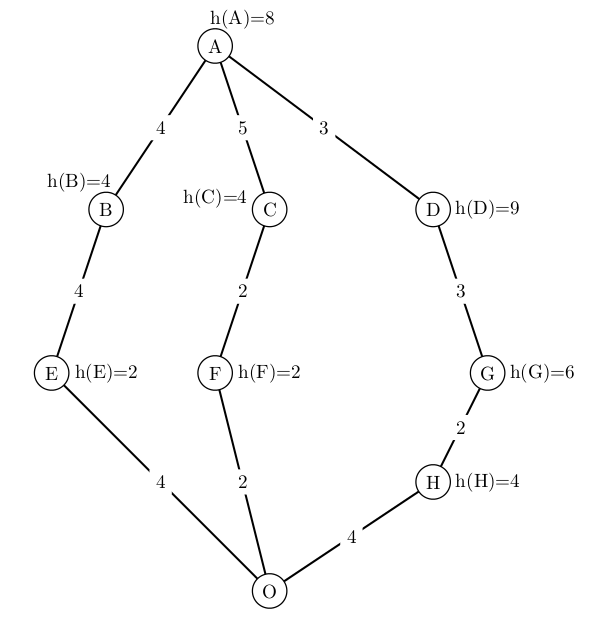
\includegraphics[width=\linewidth]{images/hachefull-left}
  %\caption{A really Awesome Image}\label{fig:image1_h1_astar}
\endminipage\hfill
\minipage{0.5\textwidth}
  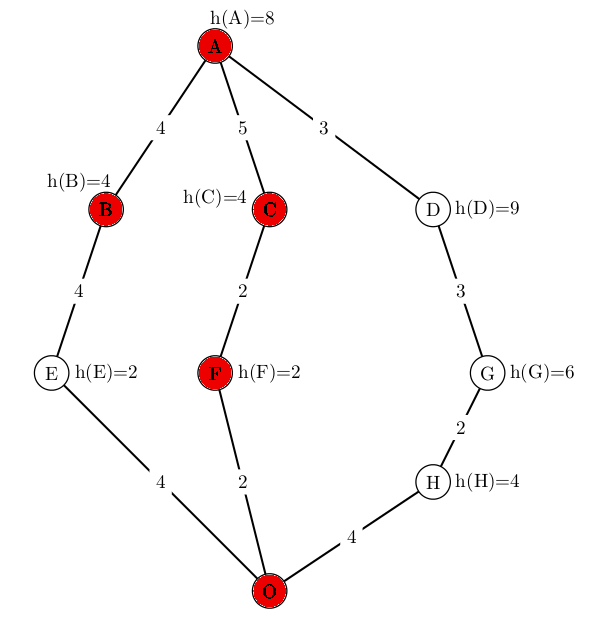
\includegraphics[width=\linewidth]{images/hachefullabcfG-right}
  %\caption{A really Awesome Image}\label{fig:image2_h2_astar}
\endminipage
\caption{The left figure shows a state space graph where the number above of each node is the heuristic value assigned by a heuristic $h_{1}$. The initial state is \texttt{A} and the goal state is \texttt{O}. The right figure shows a state space where the highlighted states are those expanded by A$\sp{*}$. }\label{fig:image_h1_astar}
\end{figure}

\begin{figure}[!htb]
\minipage{0.5\textwidth}
  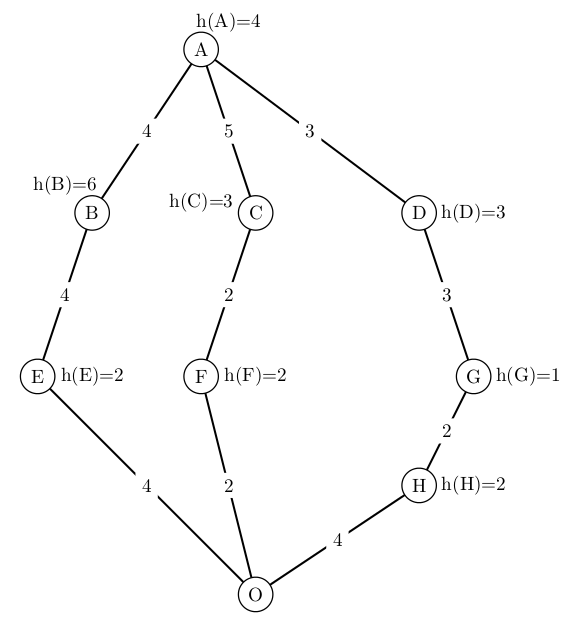
\includegraphics[width=\linewidth]{images/marvinh2full-left}
  %\caption{A really Awesome Image}\label{fig:image1_h1_astar}
\endminipage\hfill
\minipage{0.5\textwidth}
  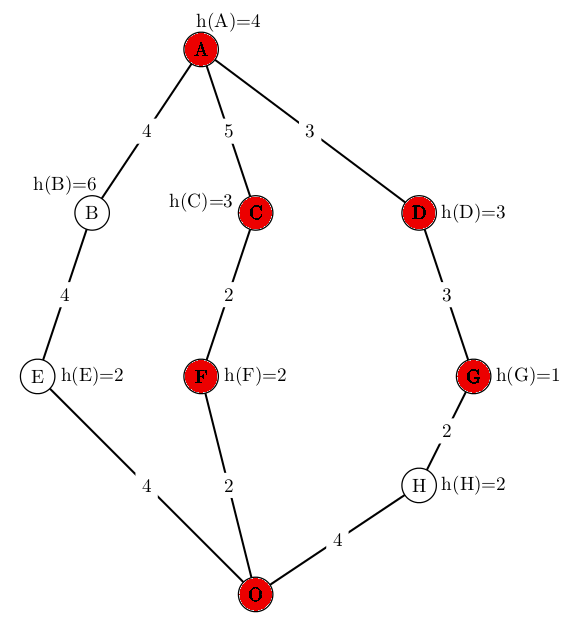
\includegraphics[width=\linewidth]{images/marvinh2fulladgcfG-right}
  %\caption{A really Awesome Image}\label{fig:image2_h2_astar}
\endminipage
\caption{The left figure shows a state space graph where the number above of each node is the heuristic value assigned by a heuristic $h_{2}$. The initial state is \texttt{A} and the goal state is \texttt{O}. The right figure shows a state space where the highlighted states are those expanded by A$\sp{*}$.}\label{fig:image_h2_astar}
\end{figure}

\begin{figure}[!htb]
\minipage{0.5\textwidth}
  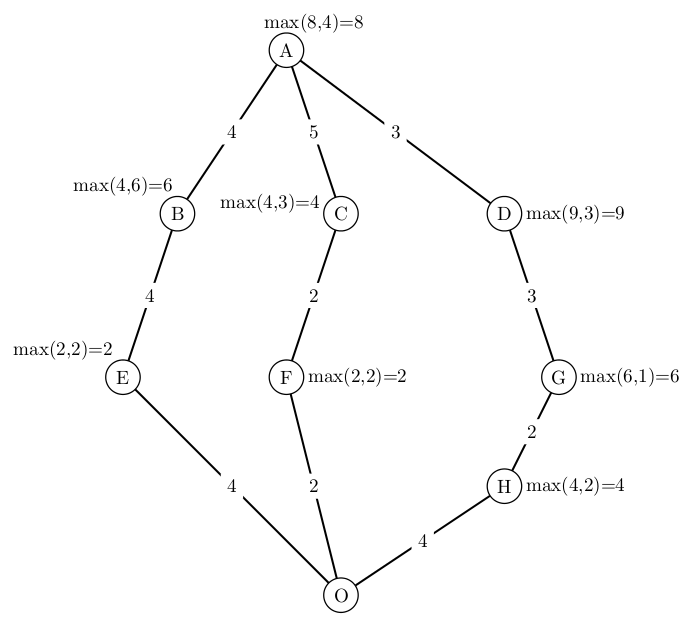
\includegraphics[width=\linewidth]{images/marvinmaxfull-left}
  %\caption{A really Awesome Image}\label{fig:image1_h1_astar}
\endminipage\hfill
\minipage{0.5\textwidth}
  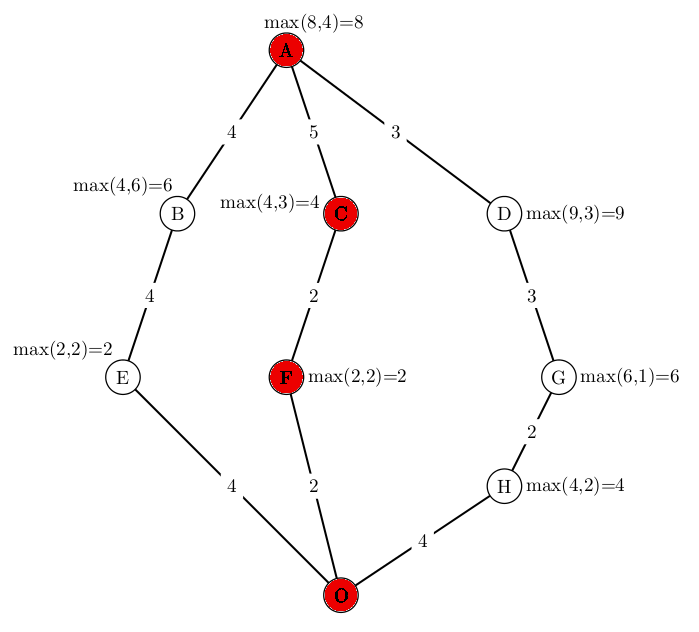
\includegraphics[width=\linewidth]{images/marvinmaxfullacfG-right}
  %\caption{A really Awesome Image}\label{fig:image2_h2_astar}
\endminipage
\caption{The left figure shows a state space graph where the number above of each node is the maximum heuristic value of $h_{1}$ and $h_{2}$. The initial state is \texttt{A} and the goal state is \texttt{O}. The right figure shows a state space where the highlighted states are those expanded by A$\sp{*}$. }\label{fig:image_maxh1h2_astar}
\end{figure}

Consider that we replace $h_{1}$ by another heuristic $h_2$, resulting in Figure \ref{fig:image_h2_astar}. The right figure shows that A$\sp{*}$ finds the optimal cost path for the problem, which has cost 9. We also observe that A$\sp{*}$ using $h_2$ expands a different set of nodes than A$\sp{*}$ using $h_1$.

One approach to take advantage of a set of heuristics $\zeta$ is to compute the maximum of all heuristics in $\zeta$. For example, given the two heuristics $h_1$ and $h_2$, the maximum of $h_1$ and $h_2$ will tend to yield a more informed heuristic than $h_1$ or $h_2$ alone. In Figure \ref{fig:image_maxh1h2_astar}, we show that A$\sp{*}$ using the maximum of heuristics values of $h_{1}$ and $h_{2}$ expands fewer nodes than each heuristic individually.

One can easily create thousands of heuristics for a problem instance. For example, each different abstraction of a problem domain results in a different \texttt{PDB} heuristic. It is possible to prove that the maximum of all heuristics in $\zeta$ cannot be less informed than the maximum of any subset of $\zeta$. However, if $\zeta$ is too large, then the resulting heuristic obtained by taking the maximum of all heuristics in $\zeta$ can be too expensive to be effective to guide search. That is why we select a subset of $\zeta$ to guide the A* search. This way we try to select the most informative heuristics in $\zeta$ while preventing the resulting maximum heuristic to be computationally expensive. 

%While taking the maximum of all heuristics in $\zeta$ will result  Using all heuristics created can 


% we need to figure it out how to take advantage of this large set of heuristics. In fact, there exist different ways to take advantage of those heuristics, however we need to take into account that if we want to use all the heuristics created by the heuristic generator, the resulting heuristic would be too expensive to guide search. This is because, the main problem involved would be the time required to evaluate all the heuristics for each node in the search tree.

%\section{Heuristic Subset}
%
%Let us suppose we have to run our meta-reasoning considering that we have a fixed amount of memory $M$. Then, one question is raised: How many heuristics our system should consider? Holte et al., (\citeyear{holte2006maximizing}) observed that maximizing over $N$ pattern databases of size $M/N$, for $N < M$, can produce a search tree size smaller than the search tree size generated by using a single pattern database of size $M$. Thus we will use heuristic generators to create a large number of heuristics to fill the amount M of memory available.
%
%Heuristic generator systems can create a large number of heuristics. Let us suppose $|\zeta| = $ 1000 heuristics were created and that our meta-reasoning for example selects $N =$ 50 heuristics. This would imply count the following number of combinations one can get from solving the combinatorial problem: $${1000\choose 50} \approx 10\sp{85} possibilities$$

In the next Chapter, we will introduce a meta-reasoning for selecting a subset of $\zeta$ to guide the A* search.

\clearpage